\section{Results}\label{results}

In this section, we demonstrate the effectiveness of the ILC algorithms presented in Section~\ref{methodology} for striking motions in table tennis. First we start with a simulation example where we study the performances of our proposed algorithm in detail.
%
\subsection{Simulation Results with Barrett WAM}

In the robotic table-tennis task where an anthropomorphic robot arm plays table-tennis with a human, the requirements for a successful performance are many. First of all, the position and velocity profile of the incoming ball need to be predicted accurately and well in advance of the hitting motion. Then a kinematics or movement primitive based reference trajectory is calculated that will intercept the ball in midair. Finally the robot arm must be controlled well: the right torques need to be found for the particular reference or they need to be acquired through learning.

The trajectories in our case are assigned in joint space, one for each of the seven joints of the simulated robot. A low-gain feedback law is calculated using LQR with the linearized nominal dynamics which stabilizes the open-loop system $\dynamics$. ILC can be applied on top of this closed-loop system, providing learning from one iteration to the next. 

%
\begin{figure}[!htb]
    \centering
    \begin{minipage}{.25\textwidth}
        \centering
        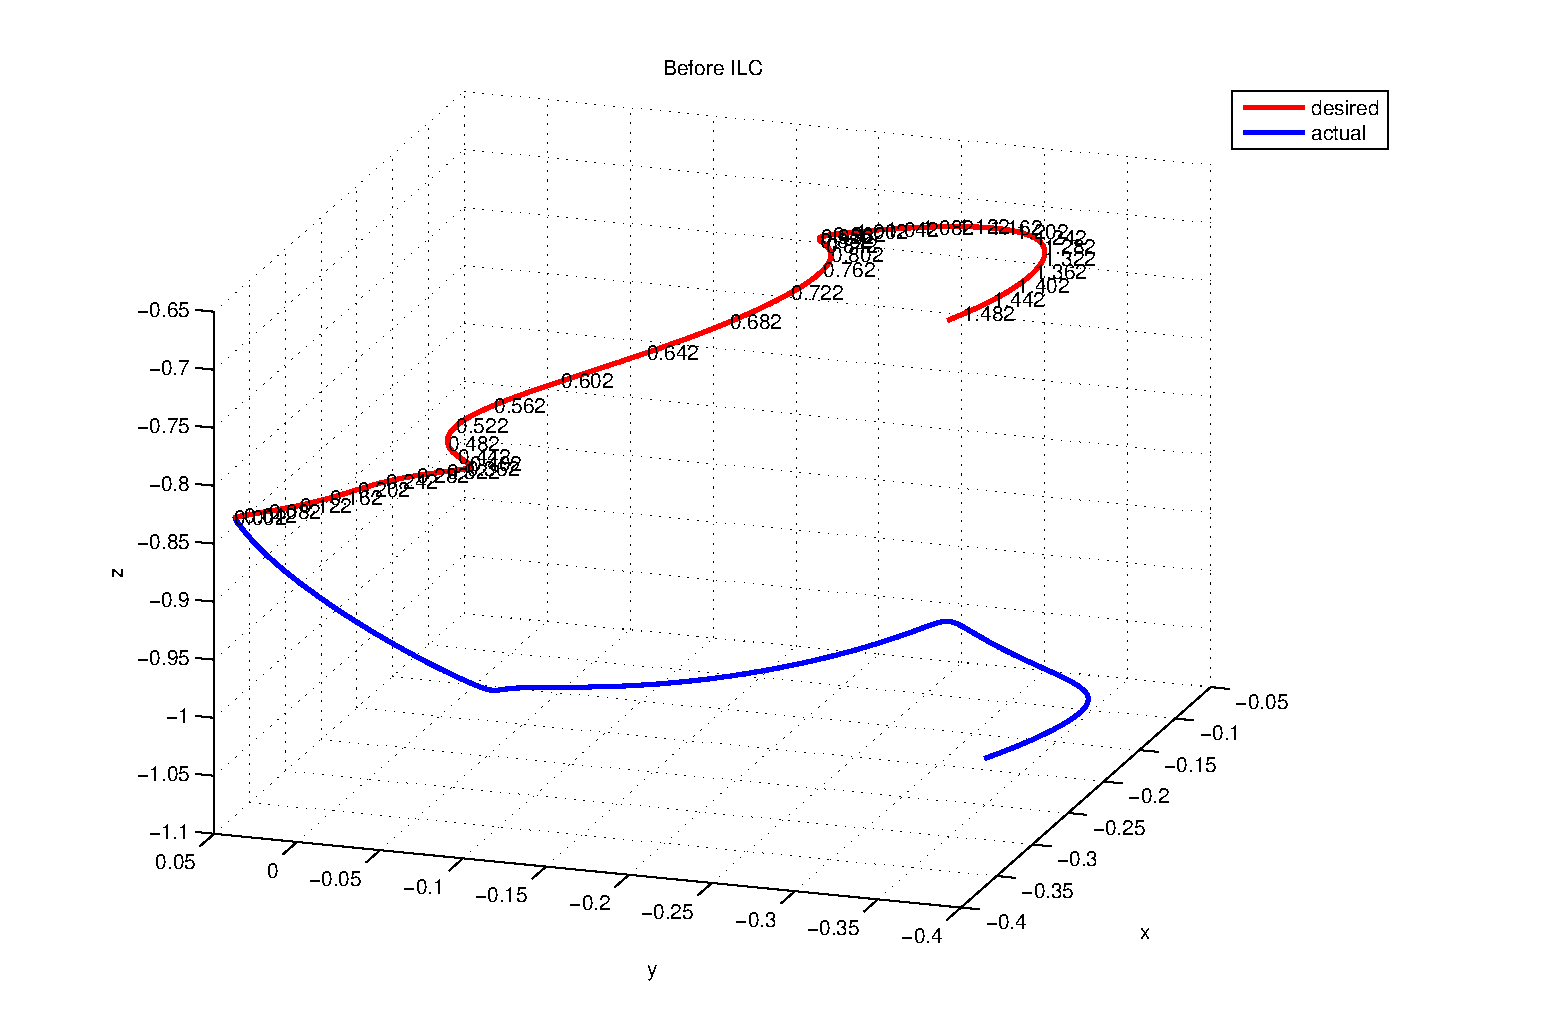
\includegraphics[width=\linewidth, height=0.15\textheight]{beforeILC.eps}
        \caption{(a)}
        \label{fig1}
    \end{minipage}%
    \begin{minipage}{.25\textwidth}
        \centering
        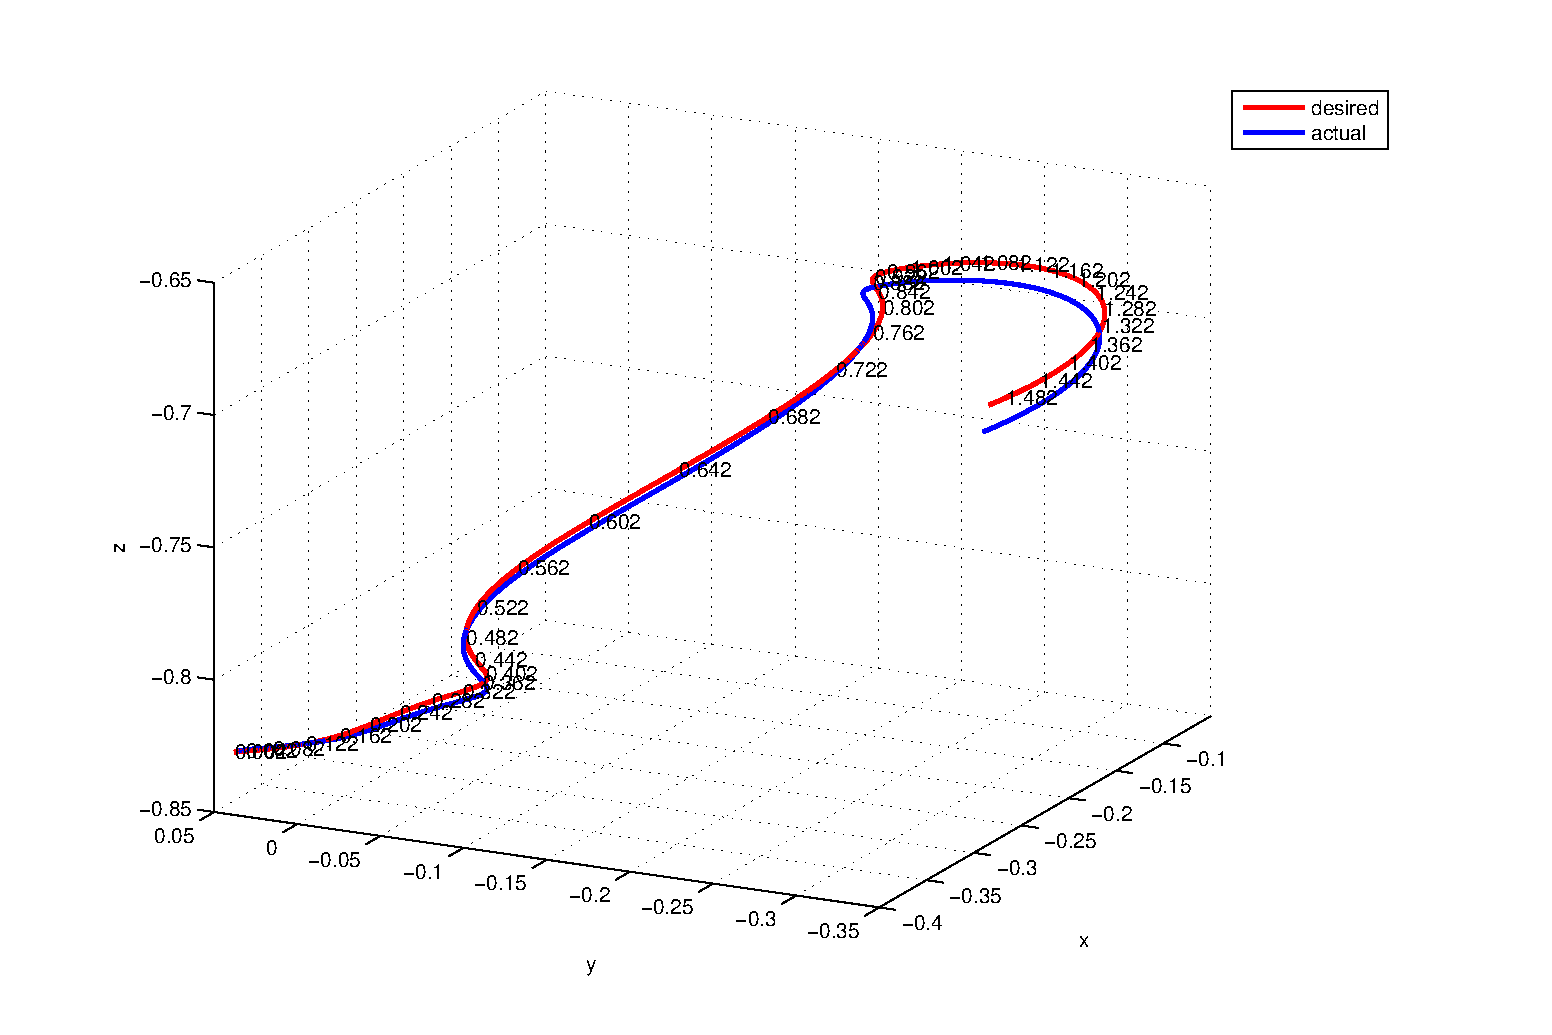
\includegraphics[width=\linewidth, height=0.15\textheight]{afterILCPseudoInv.eps}
        \caption{(b)}
        \label{fig2}
    \end{minipage}
    \begin{minipage}{.25\textwidth}
        \centering
        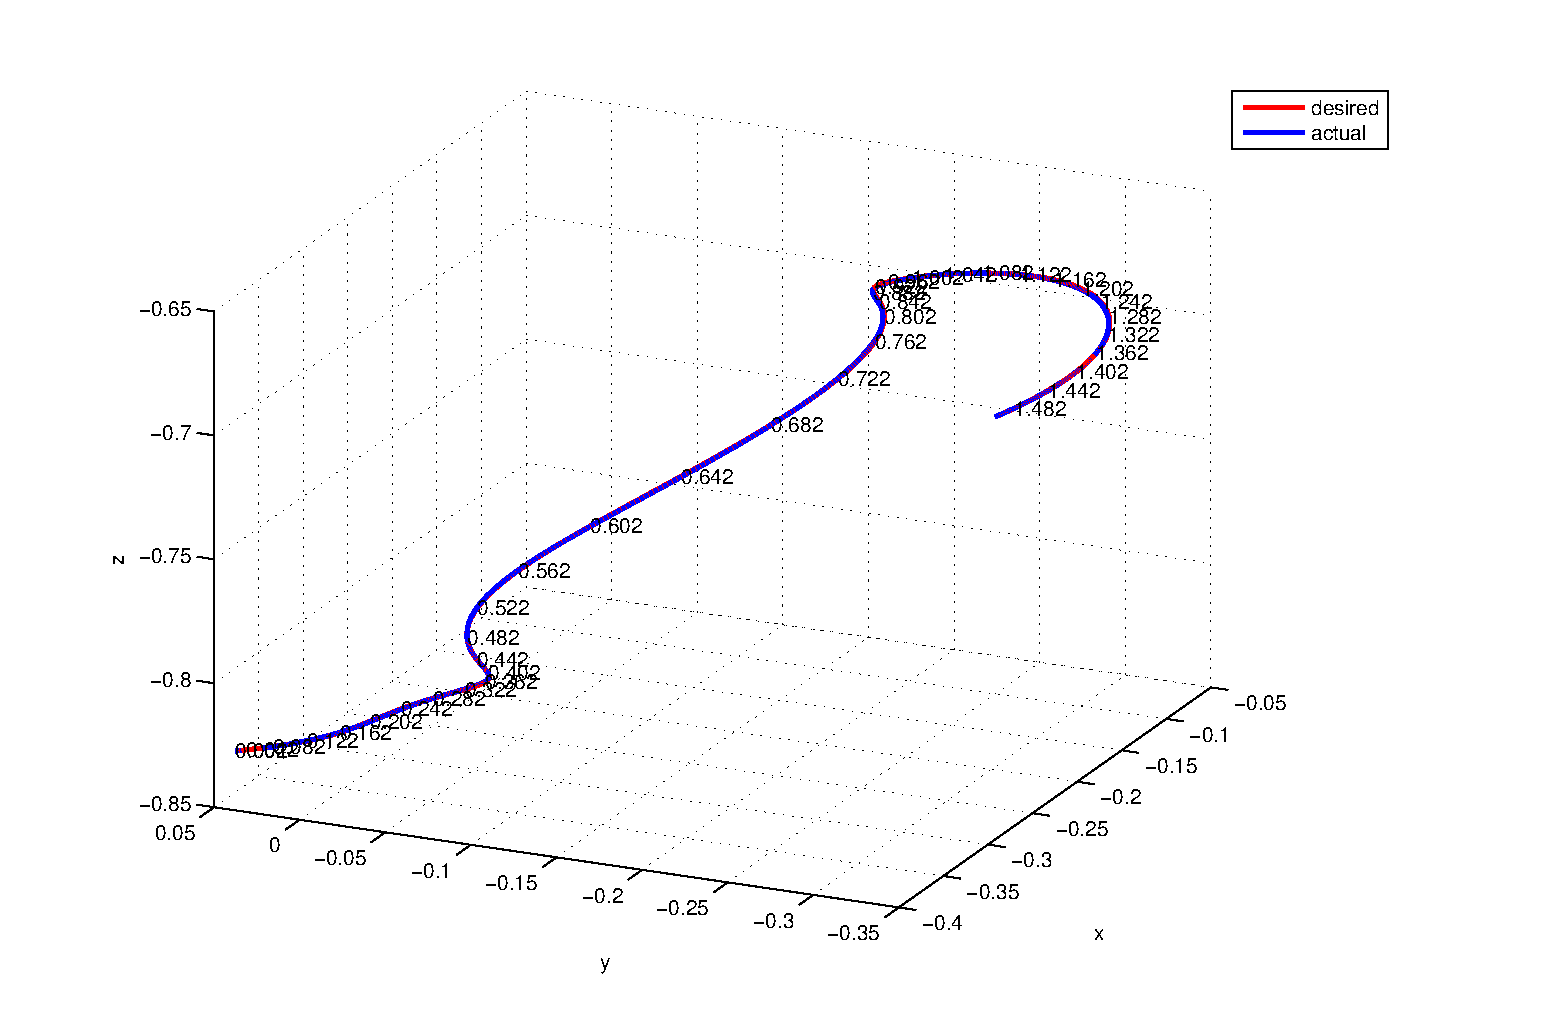
\includegraphics[width=\linewidth, height=0.15\textheight]{afterILCTLS.eps}
        \caption{(c)}
        \label{fig3}
    \end{minipage}
    \caption{Results showing the performance of trajectory tracking, before and after applying ILC (10 iterations). Reference trajectory is shown in red. Initially, in Figure~\ref{fig1}, tracking performance is poor. Final performances of pseudoinverse-based ILC and TLS-based ILC after learning are shown in Figures~\ref{fig2} and \ref{fig3} respectively. ILC with truncated pseudoinverse cannot approach the trajectory very well, and after 8 iterations starts to slowly diverge. ILC with truncated total least squares on the other hand approaches the trajectory very well, and shows excellent tracking performance that is also stable.}
\label{FigureILC}
\end{figure}

In the simulation results shown in Figure~\ref{FigureILC}, we consider a striking trajectory shown in red. Such ball-hitting trajectories in table tennis are generally composed of three parts: a preparatory phase, a hitting phase, and a relaxation phase. In the preparatory phase, the arm generally accelerates and picks up speed necessary to transfer the right momentum to the ball, intercepted in the hitting phase. The relaxation phase generally decelerates the arm and readies it for the next hitting task. 

ILC with pseudoinverse cannot approach trajectory very well, and after 8 iterations starts to slowly diverge. ILC with TLS on the other hand approaches the trajectory very well, and shows excellent tracking performance. For both methods, to be fair, we used the same truncation parameter, $\epsilon = 0.05$. This enables the pseudoinverse-based ILC to be more stable, i.e. without it ILC can show dangerous oscillations around some trajectories. However, even with truncation the pseudoinverse relies on the exactness of the model, whereas $\alg$ is inherently \emph{agnostic} to its accuracy. 

In practice we find that an additional adjustment in the form of \emph{current-iteration} ILC (\emph{CI-ILC}) 
%
\begin{equation}
\begin{aligned}
\sysInput_{k+1} &= \sysInput_k - \vec{K}_{LQR}\error_{k},\\
\end{aligned}
\label{fbILC}
\end{equation}
%
\noindent where we add the feedback from the previous iteration to the feedforward commands in the next iteration makes learning more robust. We add this current-iteration compensation to both methods in the results shown. 


\subsection{Applications in Robotic Table Tennis}

We performed the real robot experiments with a seven degree of freedom (DoF) torque-controlled custom made Barrett WAM arm capable of high speeds and accelerations.